\chapter{Implementation}
\label{chapter:implementation}

% This chapter should include design choices for my implementation. For
% example choices taken for generating relevant data for test users
% and a computational sound method for doing so. As JavaScript in browsers are
% quite inefficient it will probably be necessary to persist data at a server
% in some sort of cache. The clients could then get this data by invoking a
% single request. The result could for instance be JSON serialized. Scraping
% of such data is probably done more efficient and safer at the server side
% since multiple XMLHttpRequests in the clients for scraping and parsing could
% prove to be quite computational expensive.

As we've seen in 
\sectionref{building.on.top.of.the.web}
it's possible to build applications on top of existing web sites by creating
transparent prototype implementations. This chapter starts with an account of
what kind of navigation system we wanted to build, goes on to describe why we
decided on such navigational designs, and concludes with an explanation of how
the implementation was built\dash{}the ingredients of our implementation.

\section{Design}

% no new data. making existing data more readily available.

\section{Process}
% Prototype, exploratory
% TDD, BDD

\section{Architecture}

Our implementation basically needs to do two things:

\begin{enum}
  \item Collect existing data from various places on the \urort web site.
  \item Display this data in existing web pages on the \urort web site in
    a way that we hope will enhance navigation.
\end{enum}

We decided to use a server--client architecture so that we could offload some
of the more computationally expensive operations off the client and onto a
dedicated server. Another benefit of such an architecture is that it allows us
to cache data globally\dash{}shared by all clients. Therefore data collection
is handled on the server side, while data display obviously is handled on
the client side.

With all the pieces in place of our third party software puzzle described in
\chapterref{selection.of.third.party.software}
we present a high level view of the architecture, from the client to the
server, in
\figureref{fig.prototype.architecture}.

\begin{figure}
  \begin{whole}
    \centering
    \includegraphics[width=0.9\wholewidth]{fig_prototype_architecture}
    \caption[Prototype Architecture]{
      High level view of the overall prototype architecture.
    }
    \label{figure:fig.prototype.architecture}
  \end{whole}
\end{figure}


